\chapter{Метод главных компонент}

%\section{Введение}
%В настоящее время технология распознавания лиц имеет широкое применение в различных областях: в системах наблюдения, в системах аутентификации, в фототехнике и т.~д. В общем случае, процесс идентификации человека по изображению лица можно разделить на две части:
%\begin{enumerate}
%	\item определение местоположения лица на изображении. Различные части изображения сканируются, и каждый раз определяется степень схожести очередной части изображения с человеческим лицом.  При таком поиске лицо может быть задано структурно. Общая структура лица включает в себя овальную форму, симметрично расположенные глаза, нос, губы и т.~д.;
%	\item распознавание лиц: после обнаружения той части изображения, на которой с большой достоверностью находится только лицо человека, можно начинать процесс распознавания, т.~е. идентификации человека по изображению лица~\cite{ieee}.
%\end{enumerate}

%Метод главных компонент позволяет решить обе задачи, однако в данной работе  будет рассмотрено применение только для второй задачи~\cite{brilyuk}.

\section{Определения}

\textit{Собственный вектор матрицы} --- ненулевой вектор, умножение квадратной матрицы на который дает тот же вектор с числовым коэффициентом, называемым собственным значением~\cite{linal}.

\textit{Ковариационная матрица вектора} --- квадратная симметрическая матрица, элементами которой являются ковариации --- меры связанности всех возможных пар компонент вектора. Ковариация имеет отрицательное значение, если большие значения одной компоненты соответствуют меньшим значениям другой, и наоборот. Ковариация имеет положительное значение, если большие значения одной компоненты соответствуют большим значениям другой, и аналогично для меньших значений. Ковариация компоненты вектора самой с собой равна дисперсии \cite{teorver}. На \eqref{eq:covariance_matrix} представлен пример ковариационной матрицы для трех компонент, ковариация обозначена как Cov$(X_1, X_2)$, дисперсия обозначена как Var$(X_1, X_2)$.

\begin{equation}\label{eq:covariance_matrix}
	\Sigma = 
	\begin{bmatrix}
		\text{Var}(X_1) & \text{Cov}(X_1, X_2) & \text{Cov}(X_1, X_3) \\
		\text{Cov}(X_2, X_1) & \text{Var}(X_2) & \text{Cov}(X_2, X_3) \\
		\text{Cov}(X_3, X_1) & \text{Cov}(X_3, X_2) & \text{Var}(X_3) \\
	\end{bmatrix}
\end{equation}

\section{Алгоритм метода главных компонент}

Метод главных компонент --- один из статистических методов уменьшения размерности данных, т.~е. числа параметров, которые заданы переменными и необходимы для описания объекта. Такие методы по возможности сохраняют наибольшее количество информации и общую структуру данных~\cite{orlov, polyak}. Далее будет изложен алгоритм уменьшения размерности из $n$ в $k$:

\begin{enumerate}
	\item метод главных компонент очень чувствителен к статистическим выбросам и неточностям в данных, поэтому перед применением необходима стандартизация данных --- приведение данных к единому масштабу~\cite{polyak, zakaria}. Это можно сделать вычитанием среднего из каждой переменной и делением полученного на стандартное отклонение \cite{zakaria}:
	
	\begin{equation}\label{eq:normalization_Z1}
		Z_i = \frac{{X_i - \bar{X_i}}}{{\sigma_{X_i}}}.
	\end{equation}
	\item для уменьшения размерности данных необходимо найти переменные, которые сильно зависимы от значений друг друга, т.~е. cкоррелированные переменные. Это важно, поскольку такие переменные могут содержать излишнюю информацию, от которой можно было бы избавиться с минимальными потерями полезной информации. Чтобы понять, какие переменные скоррелированы, необходимо найти ковариационную матрицу;
	\item далее необходимо найти главные компоненты --- новые переменные, которые получаются после введения новой системы координат таким образом, что каждая следующая главная компонента максимизирует дисперсию данных относительно себя, но не коррелирует с предыдущими главными компонентами, т.~е. перпендикулярна им. Таким образом, из $n$ изначальных переменных получится $n$ главных компонент, однако последним главным компонентам будет соответствовать наименьшая дисперсия, т.~е. наименьшая изменчивость --- это означает, что эти главные компоненты содержат наименьшее количество информации и могут быть отброшены с минимальными потерями. Математически направления осей главных компонент --- это собственные векторы ковариационной матрицы, а собственные значения --- это коэффициенты, отражающие дисперсию, соответствующую этой главной компоненте. Таким образом, полученные собственные значения необходимо упорядочить по убыванию и выбрать $k$ первых собственных векторов, которые и будут новыми переменными для уменьшения размерности~\cite{orlov, polyak, zakaria};
	
	\begin{minipage}{\linewidth}
		\centering
		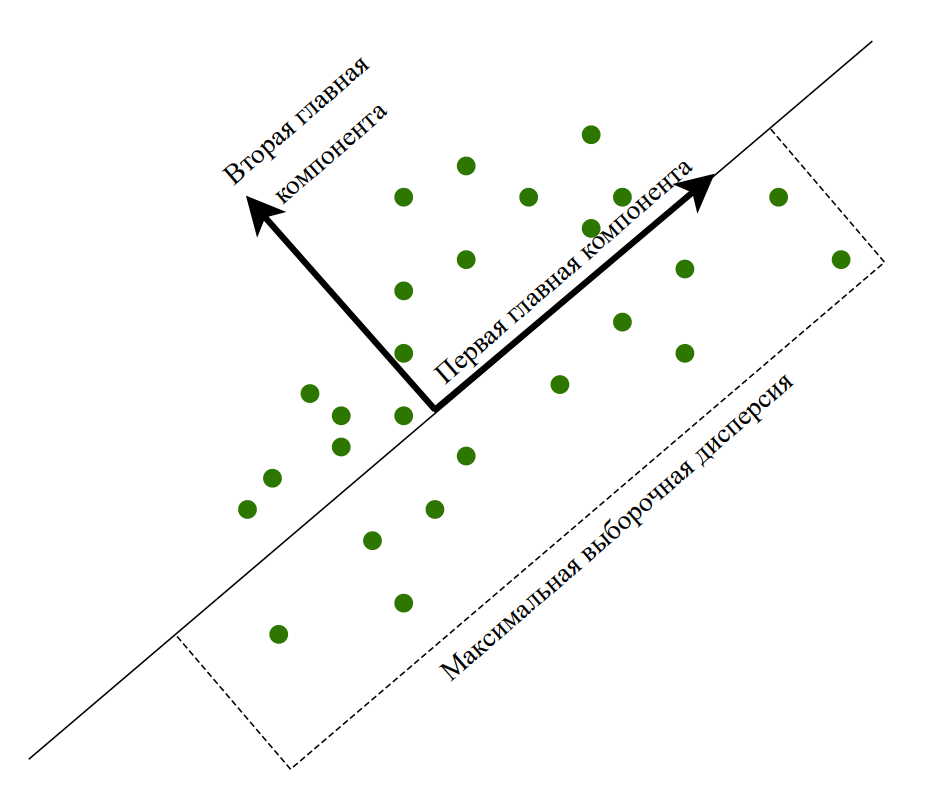
\includegraphics[width=0.9\textwidth]{img/pca1.png} 
		\captionof{figure}{Пример ввода первой и второй главных компонент}
		\label{fig:pca1}
	\end{minipage}

	
	\item На последнем шаге необходимо преобразовать данные, перейдя от исходных переменных к полученным $k$ главным компонентам. Для этого необходимо умножить транспонированную матрицу исходных данных $D$ на транспонированную матрицу главных компонент $PC$~\cite{zakaria}.
	
	\begin{equation}\label{eq:matrix_multiply}
		D^T \cdot PC^T
	\end{equation}
\end{enumerate}

\section{Применение метода главных компонент для распознавания лиц}

Для задачи распознавания человека по изображению лица метод можно применить следующим образом: входные вектора представляют собой отцентрированные (лицо должно находиться в центре изображения и занимать большую его площадь) и приведённые к единому масштабу черно-белые изображения лица $m$ на $n$ пикселов. Собственные вектора, вычисленные для всего набора изображений лиц, называются собственными лицами ($eigenfaces$). Метод главных компонент в применении к изображениям лиц так же называют методом собственных лиц. Собственные лица имеют полезное свойство, заключающееся в том, что изображение, соответствующее каждому такому вектору имеет лицеподобную форму~\cite{brilyuk, parshin}.

\begin{figure}[h]
	\centering
	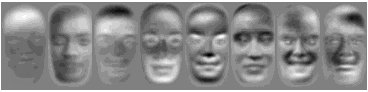
\includegraphics[width=0.85\textwidth]{img/pca2.png} 
	\caption{Пример собственных лиц~\cite{brilyuk}}
	\label{fig:pca2}
\end{figure}

Полученный один раз на обучающей выборке изображений лиц набор собственных векторов используется для кодирования всех остальных изображений лиц, которые представляются взвешенной комбинацией этих собственных векторов~\cite{parshin}. Процесс распознавания заключается в сравнении главных компонент неизвестного изображения с компонентами всех остальных изображений. Для этого обычно применяют какую-либо метрику (простейший случай --- Евклидово расстояние)~\cite{brilyuk}. 
	